\chapter{Project Planning and Timeline}

\paragraph*{}
As we have already achieved our Minimum Viable Prototype in a simulation during the previous semester, we are able to allocate the workload into two phases. The time period and the number of people allocated to the tasks are listed in the attached Gantt Chart (Figure \ref{fig:Project Gantt Chart}).

\paragraph*{}
During the first phase, our overall goal is to prepare for the hardware implementation, following the success of our previous swarm simulation. There are four major milestones for this phase: \textbf{Communication}, \textbf{SLAM in Simulation}, \textbf{Coordinated Gripping and Formation}, \textbf{and Object Detection}. 

\paragraph*{}
For \textit{communication}, we will work on implementing communication, with the target being successful data transmission and acknowledgements between three swarm members. For \textit{SLAM in Simulation}, we are planning to implement either Graph-SLAM or Cartographer in our system to perform localization and mapping. For \textit{Coordinated Gripping and Formation}, this comprises the gripper design, and a robust and resilient path finding algorithm, with the ability to avoid obstacles and collisions within the swarm. For \textit{Object Detection}, using both camera and Lidar to perform object detection and measurements is required. Additionally, pose estimation will be included in that milestone.

\paragraph*{}
Throughout the second phase, we will aim to combine the whole system to be one single swarm system. The major milestones for the second phase are: \textbf{Hardware}, \textbf{Movement after Gripping}, and \textbf{Testing and Evaluation}.

\paragraph*{}
\textit{Hardware} will be worked on in parallel with a lot of the prior steps, since our main focus for this semester is the hardware integration of the swarm for practical demonstration purposes. \textit{Movement after Gripping} is the action of the swarm after they have latched onto an object. To be precise, it is the coordinated movement to a specific location alongside the grabbed object. Finally, \textit{Testing and Evaluation} will be performed. In this duration, we will perform evaluations catered to our design criteria to evaluate whether our swarm system meets our objectives or not. This is a process that will yield feedbacks and eventually offer rooms for improvement for the completed swarm system.

\begin{figure}
    \centering
    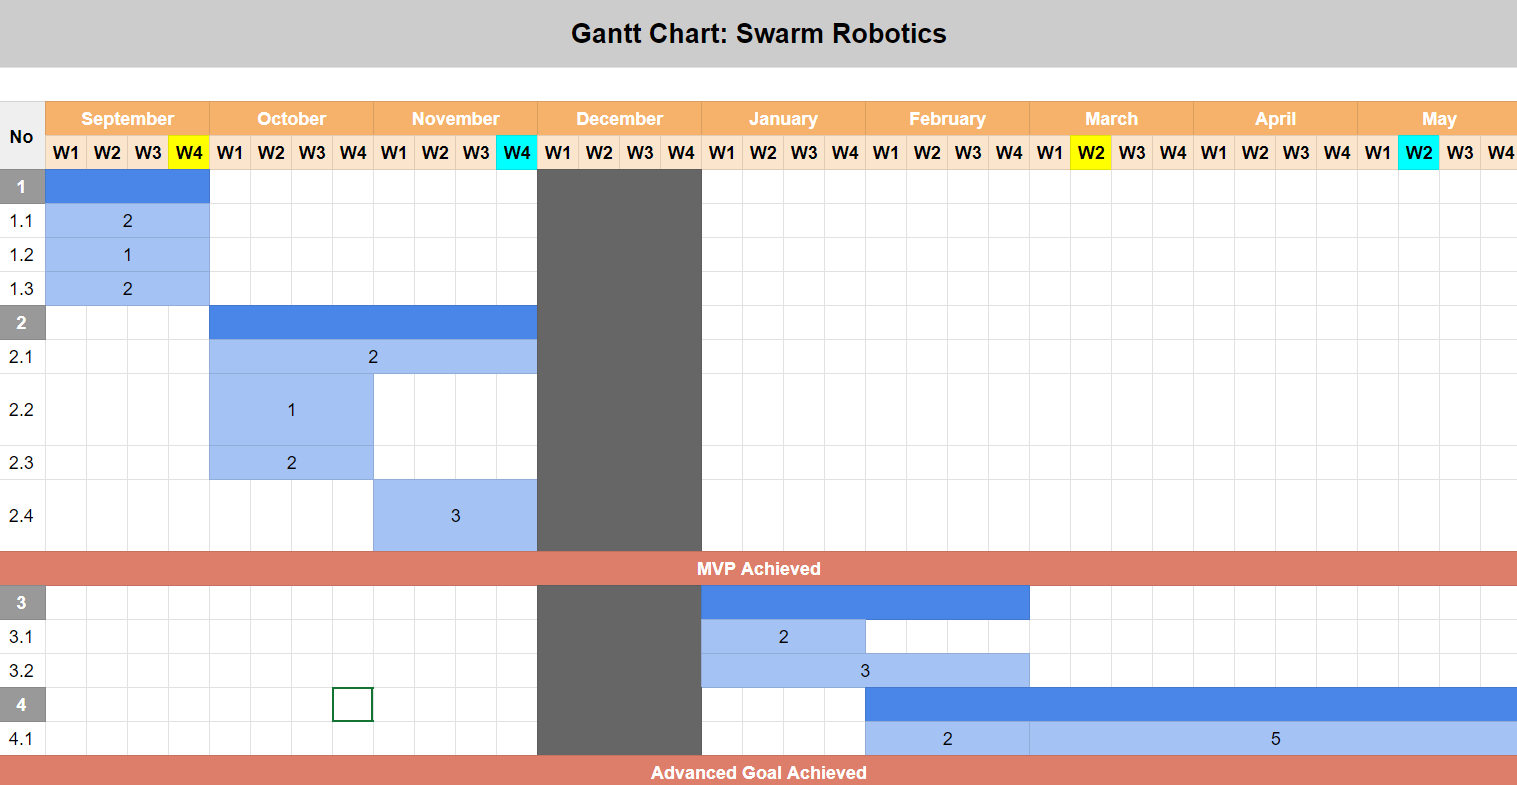
\includegraphics[width=1\linewidth]{assets/images/timeline/gantt_chart.png}
    \caption{Gantt Chart}
    \label{fig:Project Gantt Chart}
\end{figure}

\begin{enumerate}
    \item Preparation for Hardware Implementation
    \begin{enumerate}[label=1.\arabic*]
        \item Communication in the swarm
        \item Simple Simultaneous Localization and Mapping (SLAM) in Simulation
        \item Coordinated Gripping and Formation
        \item Object detection
    \end{enumerate}
    \item Moving Towards a Complete Swarm
    \begin{enumerate}[label=2.\arabic*]
        \item Hardware
        \item Movement after Gripping
        \item Testing and Evaluation
    \end{enumerate}
\end{enumerate}
